\section{Propuesta a desarrollar}
\label{sec:Propuesta a desarrollar}
    % Parrafo 1
        El proyecto propuesto consiste en el desarrollo de un sistema de monitoreo poblacional basado en 
            la implementaci\'on de un aut\'omata en un modelo bidimensional no lineal. En este caso, 
            como mencionamos anteriormente, el algoritmo esta basado en el modelo de Physarum Polycephalum.
            Este modelo es un organismo unicelular que se comporta como un aut\'omata celular,
            y es capaz de resolver problemas de optimizaci\'on y ruteo.
        \vskip 0.5cm
    % Parrafo 2
        A su vez, el sistema propuesto se basa en la utilizaci\'on de robots aut\'onomos, los cuales 
            se encargar\'an de recolectar informaci\'on de la poblaci\'on y de los entornos en los que 
            se encuentran. Estos robots estar\'an equipados con c\'amaras y sensores que les permitir\'an 
            detectar y clasificar entidades poblacionales. Adem\'as, los robots estar\'an conectados a 
            una red de comunicaci\'on que les permitir\'a compartir informaci\'on en tiempo real.
        \vskip 0.5cm
    % Parrafo 3
        El sistema funcionar\'a de la siguiente manera: los robots aut\'onomos recibir\'an la ruta a seguir 
            por parte de nuestro simulador del Physarum Polycephalum, el cual se encargar\'a de determinar
            la ruta \'optima para recolectar informaci\'on de la poblaci\'on. Una vez que los robots
            recolecten la informaci\'on, esta ser\'a enviada a un servidor central, el cual se encargara
            de procesar la informaci\'on y de generar reportes en tiempo real.
        \vskip 0.5cm
    % Parrafo 4
        La implementaci\'on de este sistema permitir\'a a los investigadores y a las autoridades locales
            monitorear poblaciones de manera eficiente y en tiempo real. Adem\'as, el sistema permitir\'a
            la detecci\'on de cambios en las poblaciones y en los entornos en los que se encuentran.
        \vskip 0.5cm
    % Parrafo 5
        Por ello tendremos principalmente dos 'productos' a desarrollar, el primero ser\'a el simulador
            del Physarum Polycephalum, el cual ser\'a un sistema que permitir\'a determinar rutas \'optimas
            para recolectar informaci\'on de la poblaci\'on. El segundo producto ser\'a el sistema de 
            monitoreo poblacional, el cual ser\'a un sistema que permitir\'a a los robots aut\'onomos 
            recolectar informaci\'on de la poblaci\'on y de los entornos en los que se encuentran.
        \vskip 0.5cm
    % Parrafo 6
        Se detallar\'a la implementaci\'on de estos sistemas en las siguientes secciones.
    \subsection{Requerimientos} % (fold)

    % Parrafo 1
    Para el desarrollo de nuestro Trabajo Terminal (TT), es necesario establecer los requerimientos 
        que debe cumplir el robot que simular\'a el comportamiento del Physarum Polycephalum. 
        En las siguientes secciones, se describir\'an los requerimientos funcionales y no funcionales que 
        se deben cumplir en nuestro Trabajo Terminal (TT).
    \vskip 0.5cm
    \subsubsection{Requerimientos funcionales} % (fold)

    En esta secci\'on se presentan los requerimientos funcionales que definen las 
        caracter\'isticas y capacidades espec\'ificas que el sistema debe proporcionar 
        para cumplir su prop\'osito en el contexto de simulaci\'on y monitoreo de rutas 
        automatizadas. Estos requerimientos aseguran que el sistema cumpla con las 
        funciones clave necesarias para la interacci\'on y operaci\'on de la simulaci\'on.
        Los requerimientos funcionales se listan en el Cuadro \ref{tab:requerimientos_funcionales}.
    \vskip 0.5cm
    \begin{table}[h!]
        \centering
        \begin{tabular}{|c|c|p{12cm}|}
        \hline
        \textbf{ID} & \textbf{Nombre} & \textbf{Requerimiento Funcional} \\
        \hline
        RF1 & Seleccionar  & Permitir al usuario seleccionar estados en el simulador mediante el teclado y el rat\'on. \\
        \hline
        RF2 & Colocar & Posibilitar la colocaci\'on de los estados inicial y final en el lienzo antes de iniciar la simulaci\'on. \\
        \hline
        RF3 & Iniciar & Habilitar la simulaci\'on de rutas al presionar la tecla ENTER. \\
        \hline
        RF4 & Cargar & Proveer la opci\'on de cargar un mapa o imagen en el lienzo para definir el entorno inicial de la simulaci\'on. \\
        \hline
        RF5 & Visualizar & Mostrar la ruta generada en tiempo real durante la simulaci\'on. \\
        \hline
        \end{tabular}
        \caption{Requerimientos funcionales del sistema}
        \label{tab:requerimientos_funcionales}
    \end{table}
    \subsubsection{Requerimientos no Funcionales}

    En esta secci\'on se describen los requerimientos no 
        funcionales, los cuales establecen los criterios de calidad y 
        desempe\~no que el sistema debe cumplir para garantizar una operaci\'on 
        robusta, eficiente y compatible en distintos entornos. Estos 
        requerimientos no funcionales aseguran que el sistema sea eficiente, 
        adaptable y compatible, proporcionando una experiencia de usuario 
        satisfactoria. Los requerimientos no funcionales se detallan en el Cuadro \ref{tab:requerimientos_no_funcionales}.
    \vskip 0.5cm
    \begin{table}[h!]
        \centering
        \begin{tabular}{|c|p{12cm}|}
        \hline
        \textbf{ID} & \textbf{Requerimiento No Funcional} \\
        \hline
        RNF1 & El sistema debe ser eficiente en t\'erminos de tiempo de simulaci\'on para optimizar el tiempo de generaci\'on de cada iteraci\'on. \\
        \hline
        RNF2 & El sistema debe ser capaz de manejar simulaciones en mapas grandes y con obst\'aculos sin p\'erdida significativa de rendimiento. \\
        \hline
        RNF3 & El sistema debe ser compatible tanto con sistemas operativos Windows como Linux. \\
        \hline
        \end{tabular}
        \caption{Requerimientos No Funcionales del Sistema}
        \label{tab:requerimientos_no_funcionales}
    \end{table}
    \clearpage
\subsection{Diagramas} % (fold)
\label{sub:Diagramas}


    %Parrafo
        En esta secci\'on se presentan todos los diagramas necesarios para la implementaci\'on del sistema propuesto.
        En primer lugar, se presenta un diagrama de arquitectura del sistema propuesto, el cual muestra la interacci\'on 
        entre los diferentes componentes del sistema. 
        \vskip 0.5cm
        % FIgura 
            \begin{figure}[htbp]
                \centering
                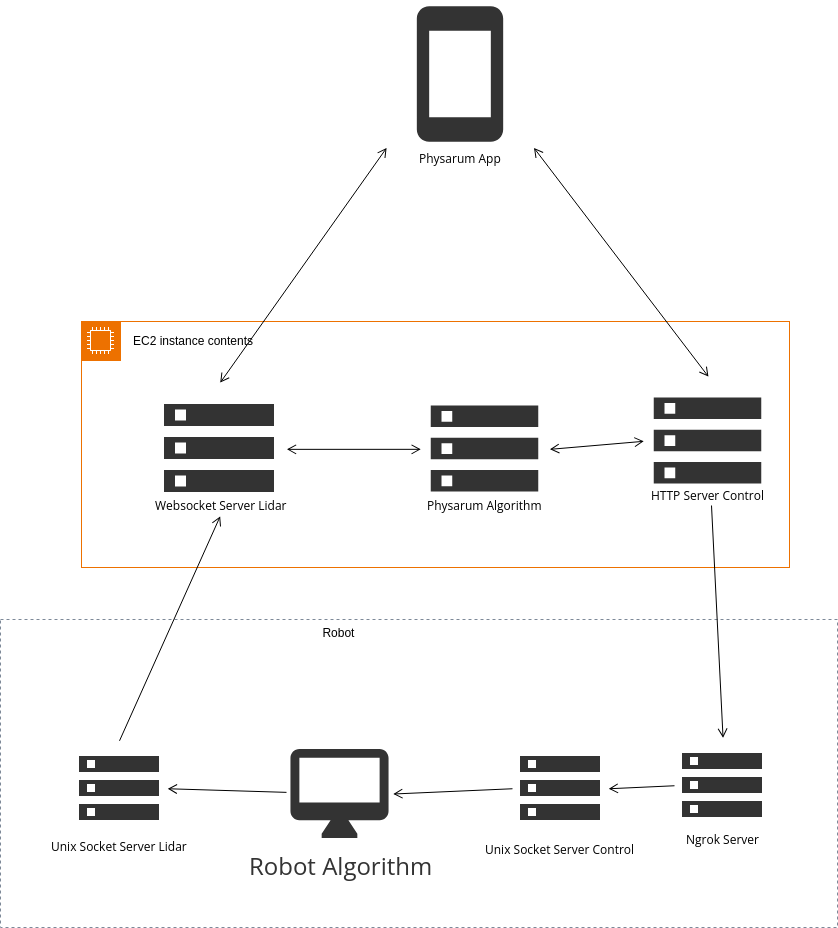
\includegraphics[width=0.8\textwidth]{images/desarrollo/diagramas/ArquitecturaSistema.png}
                \caption{Diagrama de arquitectura del sistema propuesto.}
                \label{fig:ArquitecturaSistema}
            \end{figure}
        %Parrafo
        \vskip 0.5cm
        Como se muestra en la Figura \ref{fig:ArquitecturaSistema}, el sistema mostrado en el diagrama representa una arquitectura distribuida implementada para el control remoto 
        de un robot mediante un algoritmo basado en \textbf{Physarum polycephalum} y la utilizaci\'on de datos obtenidos por un sensor LiDAR. 
        La arquitectura se compone de tres capas principales: la capa de la aplicaci\'on m\'ovil, la capa de procesamiento en la nube 
        y la capa f\'isica del robot.
        \vskip 0.5cm
        La \textbf{Physarum App} es la interfaz de usuario a trav\'es de la cual se env\'ian los comandos al sistema, 
        los cuales son gestionados por un servidor Protocolo de Transferencia de Hipertexto (Hypertext Transfer Protocol, HTTP) ubicado en una instancia EC2 de Amazon Web Services. Esta instancia 
        contiene tres servidores: un servidor HTTP que recibe los comandos de control, un servidor WebSocket que maneja la 
        recepci\'on de los datos del sensor LiDAR enviados desde el robot, y el n\'ucleo del sistema, el algoritmo de \textbf{Physarum},
        encargado de procesar esta informaci\'on para la toma de decisiones en tiempo real sobre el comportamiento del robot.
        \vskip 0.5cm
        En la capa f\'isica, el robot est\'a controlado 
        mediante dos servidores Unix Socket. El \textbf{Unix Socket Server LiDAR} recibe 
        y transmite los datos del sensor LiDAR al servidor WebSocket en la instancia EC2, 
        mientras que el \textbf{Unix Socket Server Control} se encarga de recibir los comandos procesados y enviarlos al robot. 
        Adem\'as, se utiliza un servidor Ngrok que permite la conexi\'on remota segura, facilitando el control del robot desde 
        la aplicaci\'on m\'ovil.
        \vskip 0.5cm
        Esta arquitectura distribuida permite la integraci\'on fluida de los componentes del sistema, 
        asegurando una correcta interacci\'on entre los datos sensoriales, el procesamiento en la nube y el control 
        remoto del robot.
        \vskip 0.5cm
        Despu\'es de la presentaci\'on de la arquitectura del sistema, se presentan los diagramas de flujo de las Figuras
        \ref{fig:FlujoSimulador} - \ref{fig:FlujoApp}.
        \vskip 0.5cm
        % FIgura 
            \begin{figure}[htbp]
                \centering
                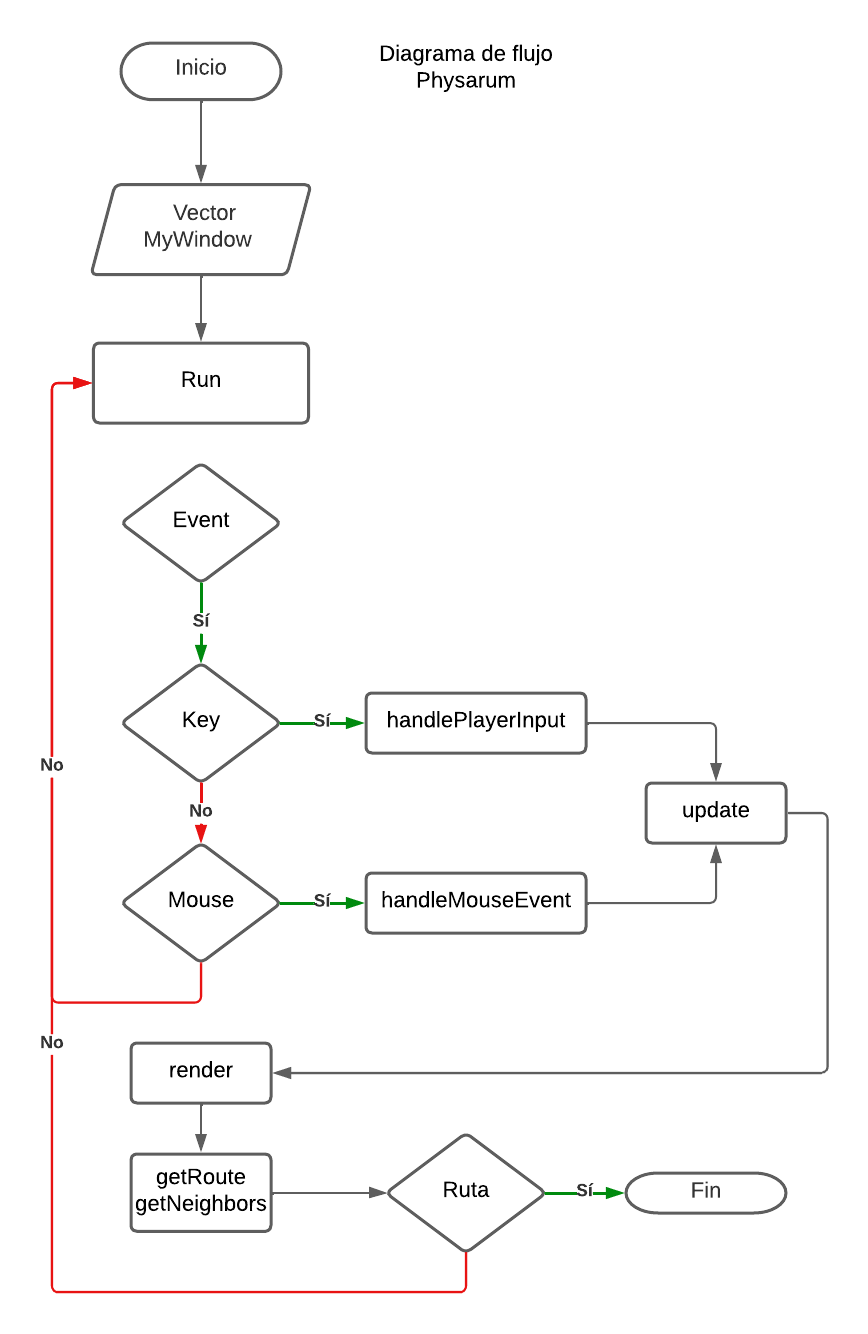
\includegraphics[width=0.5\textwidth]{images/desarrollo/diagramas/FlujoSim.png}
                \caption{Diagrama de flujo del simulador de \textbf{Physarum polycephalum}.}
                \label{fig:FlujoSimulador}
            \end{figure}
        %Parrafo
        \vskip 0.5cm

        \vskip 0.5cm
        % FIgura 
            \begin{figure}[htbp]
                \centering
                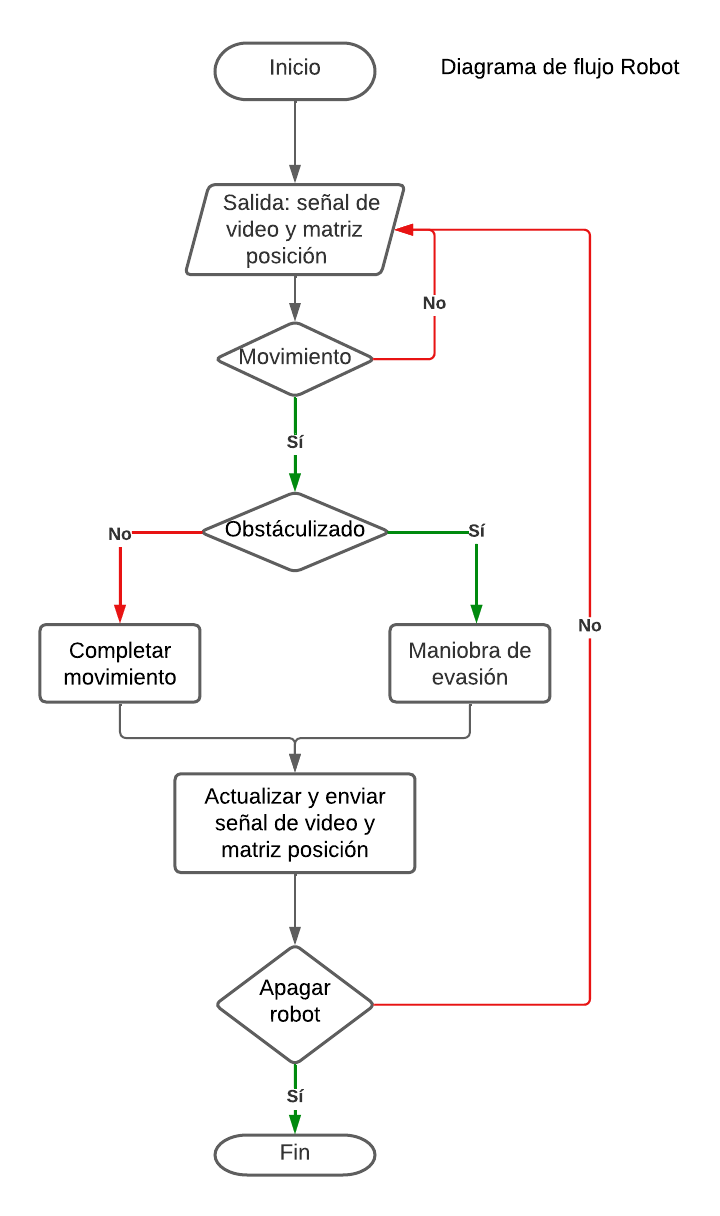
\includegraphics[width=0.5\textwidth]{images/desarrollo/diagramas/FlujoRobot.png}
                \caption{Diagrama de flujo del sistema del robot aut\'onomo.}
                \label{fig:FlujoRobot}
            \end{figure}
        %Parrafo
        \vskip 0.5cm
        \vskip 0.5cm
        % FIgura 
            \begin{figure}[htbp]
                \centering
                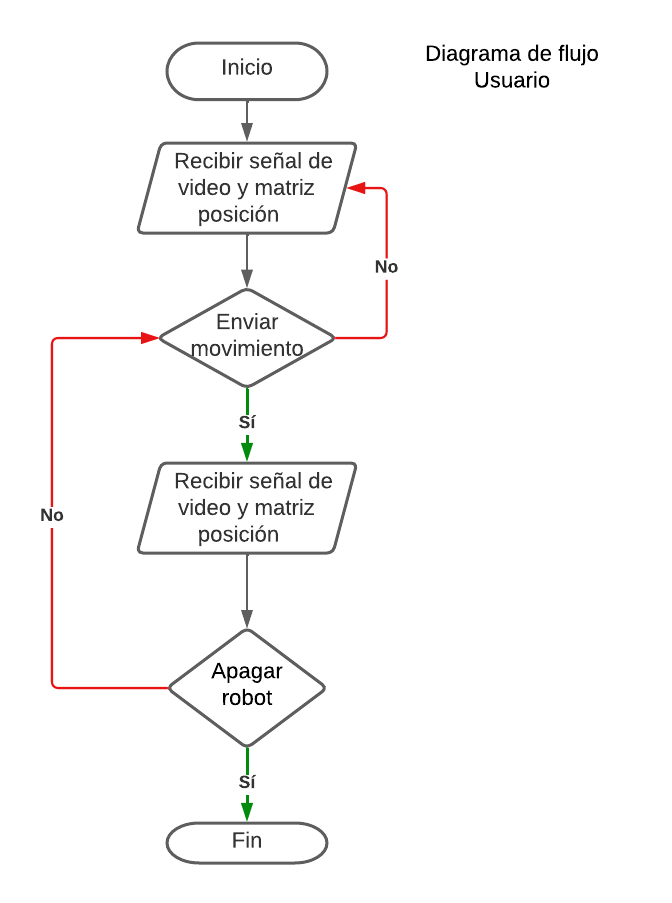
\includegraphics[width=0.5\textwidth]{images/desarrollo/diagramas/FlujoApp.png}
                \caption{Diagrama de flujo de la aplicaci\'on m\'ovil.}
                \label{fig:FlujoApp}
            \end{figure}
        %Parrafo
        \vskip 0.5cm
        \clearpage
        Despu\'es de la presentaci\'on de los diagramas de flujo, en la Figura \ref{fig:Clases} se presenta el diagrama de clases del sistema propuesto.
        \vskip 0.5cm
        % FIgura 
            \begin{figure}[htbp]
                \centering
                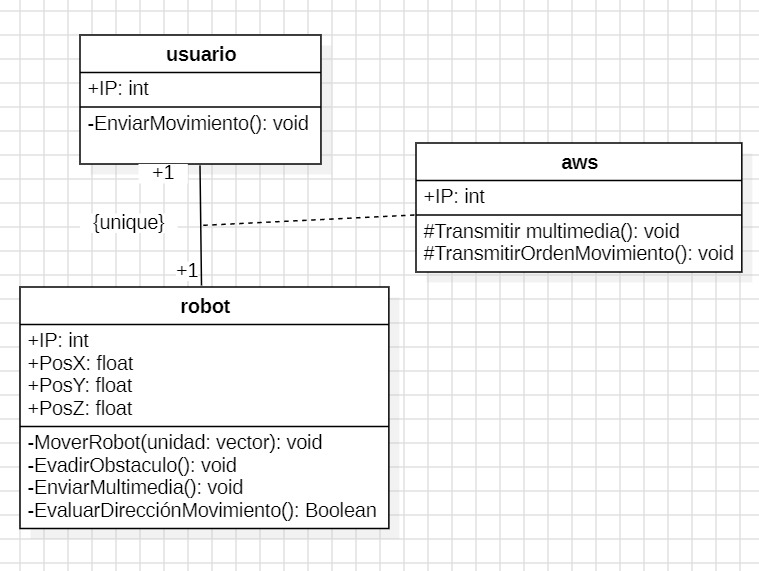
\includegraphics[width=0.8\textwidth]{images/desarrollo/diagramas/Clases.jpeg}
                \caption{Diagrama de clases del sistema propuesto.}
                \label{fig:Clases}
            \end{figure}
        %Parrafo
        \vskip 0.5cm
        El diagrama de clases muestra la interacci\'on entre el usuario, el robot y un servidor en Amazon Web Services (AWS). 
        El \textbf{usuario} tiene un atributo para su direcci\'on IP y un m\'etodo \textit{EnviarMovimiento()} 
        que le permite enviar \'ordenes al \textbf{robot}. Este \'ultimo, con atributos para su IP y su posici\'on en los ejes X, Y 
        y Z, tiene m\'etodos para moverse (\textit{MoverRobot()}), evitar obst\'aculos (\textit{EvadirObstaculo()}), 
        transmitir multimedia (\textit{EnviarMultimedia()}) y evaluar su direcci\'on de movimiento (\textit{EvaluarDirecci\'onMovimiento()}).
        \vskip 0.5cm
        El \textbf{servidor en AWS} cuenta con m\'etodos para transmitir multimedia y \'ordenes de movimiento hacia el robot. 
        El servidor act\'ua como intermediario entre el robot y el sistema, facilitando la transmisi\'on de datos y el control 
        remoto de manera segura y eficiente. El sistema asegura una comunicaci\'on \'unica y directa entre cada usuario y su robot, 
        manteniendo una interacci\'on fluida y controlada.
        % Parrafo
        \vskip 0.5cm
        En la figura \ref{fig:CasosDeUso} se presenta el diagrama de casos de usos del sistema propuesto.
        \vskip 0.5cm
        % FIgura 
            \begin{figure}[htbp]
                \centering
                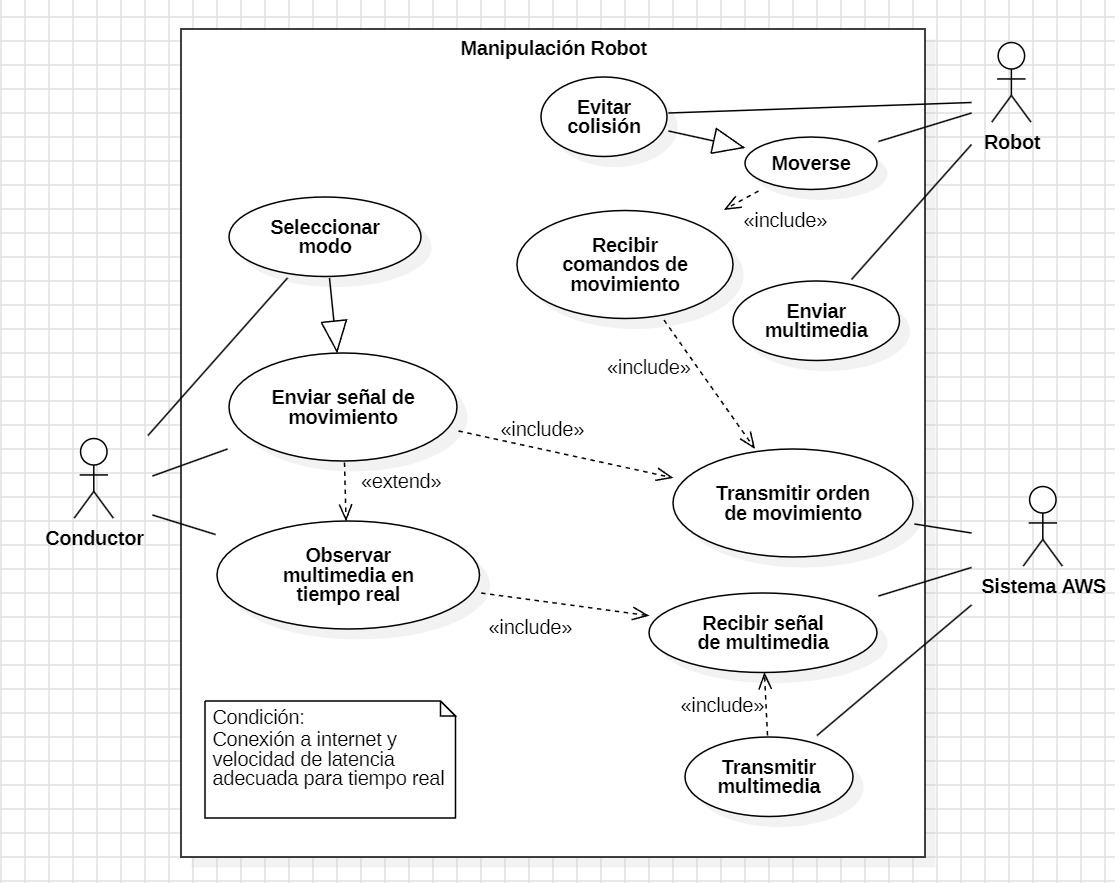
\includegraphics[width=0.8\textwidth]{images/desarrollo/diagramas/CasosDeUso.jpeg}
                \caption{Diagrama de casos de uso del sistema propuesto.}
                \label{fig:CasosDeUso}
            \end{figure}
        %Parrafo
        \vskip 0.5cm
        \clearpage
        Y el Cuadro \ref{tab:casosdesc} muestra la descripci\'on del caso de uso \textbf{Manipulaci\'on del Robot}.
        \begin{longtable}{|p{4cm}|p{10cm}|}
        \caption{Descripci\'on del Caso de Uso: Manipulaci\'on del Robot} \label{tab:casosdesc} \\
        \hline
        \textbf{Identificador}     & CU-01 Manipulaci\'on del Robot \\ \hline
        \textbf{Descripci\'on}       & El conductor controla los movimientos del robot, seleccionando el modo de operaci\'on, enviando comandos de movimiento y observando la transmisi\'on multimedia en tiempo real mientras AWS transmite las \'ordenes y multimedia. \\ \hline
        \textbf{Actores}           & Conductor, Robot, Sistema AWS \\ \hline
        \textbf{Precondiciones}    & 
        \begin{itemize}
            \item El sistema debe estar conectado a internet.
            \item La latencia de la red debe ser adecuada para la transmisi\'on en tiempo real.
        \end{itemize} \\ \hline
        \textbf{Postcondiciones}   & 
        \begin{itemize}
            \item El robot ejecuta las \'ordenes de movimiento enviadas por el conductor.
            \item El conductor puede observar la transmisi\'on multimedia en tiempo real.
        \end{itemize} \\ \hline
        \textbf{Secuencia Normal}  & 
        \begin{enumerate}
            \item El conductor selecciona el modo de operaci\'on del robot.
            \item El conductor env\'ia una se\~nal de movimiento.
            \item El sistema AWS recibe la se\~nal y la transmite al robot.
            \item El robot recibe la se\~nal y ejecuta el movimiento seg\'un las instrucciones.
            \item El robot evita colisiones mientras se mueve.
            \item El robot transmite la se\~nal multimedia en tiempo real.
            \item El conductor observa la multimedia transmitida en tiempo real.
        \end{enumerate} \\ \hline
        \textbf{Excepciones}       & 
        \begin{enumerate}
            \item Si la conexi\'on a internet se pierde o es inestable, el sistema notifica al conductor sobre la interrupci\'on en la transmisi\'on.
            \item Si el robot detecta un obst\'aculo ineludible, detiene su movimiento y espera nuevas instrucciones.
        \end{enumerate} \\ \hline
        \textbf{Rendimiento}       & 
        \begin{itemize}
            \item El sistema debe procesar las \'ordenes de movimiento en menos de 1 segundo.
            \item La transmisi\'on de la se\~nal multimedia debe tener un m\'aximo de 300ms de latencia.
        \end{itemize} \\ \hline
        \textbf{Frecuencia}        & Se espera que este caso de uso se realice continuamente durante la operaci\'on del robot. \\ \hline
        \textbf{Importancia}       & Vital \\ \hline
        \textbf{Urgencia}          & Inmediata, ya que el sistema debe responder en tiempo real. \\ \hline
        \textbf{Comentarios}       & El sistema depende de la calidad de la conexi\'on a internet para mantener la comunicaci\'on en tiempo real entre el conductor y el robot. \\ \hline
        \end{longtable}

        \clearpage

        Finalmente, en la Figura \ref{fig:Secuencia} se presenta el diagrama de secuencia del sistema propuesto.
        \vskip 0.5cm
        % FIgura 
            \begin{figure}[htbp]
                \centering
                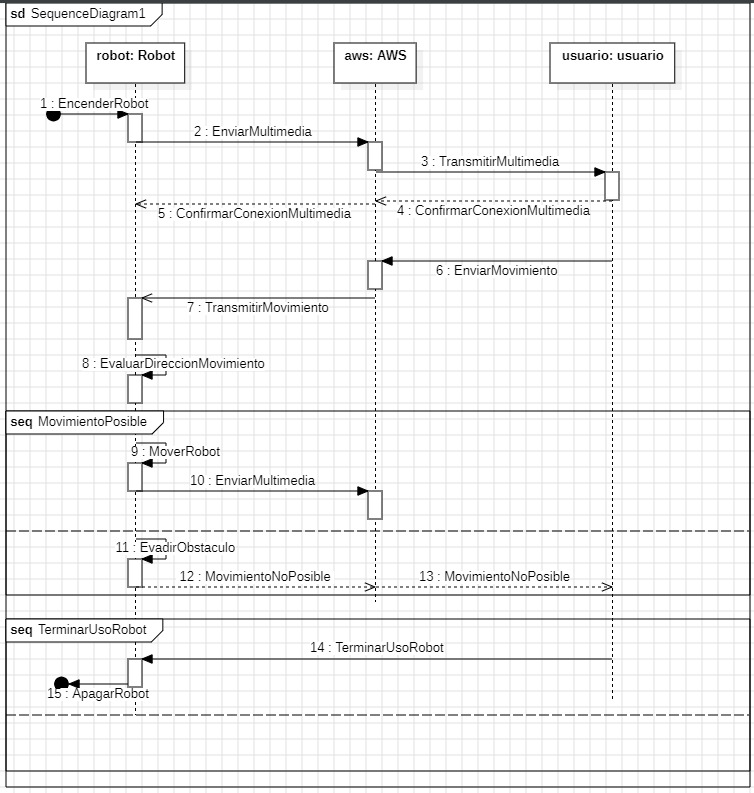
\includegraphics[width=0.8\textwidth]{images/desarrollo/diagramas/Secuencia.jpeg}
                \caption{Diagrama de secuencia del sistema propuesto.}
                \label{fig:Secuencia}
            \end{figure}
        %Parrafo
        \vskip 0.5cm
        El diagrama de secuencia muestra la interacci\'on entre el \textbf{robot}, el \textbf{servidor AWS}, y el \textbf{usuario}. Comienza cuando 
        el usuario enciende el robot, lo que desencadena la transmisi\'on de multimedia desde el robot hacia AWS, que luego retransmite 
        al usuario. Tras esto, se confirma la conexi\'on de multimedia entre el robot y AWS, asegurando que el sistema est\'e listo para 
        recibir comandos.
        \vskip 0.5cm
        El usuario puede entonces enviar \'ordenes de movimiento al robot a trav\'es de AWS. El robot eval\'ua la direcci\'on del movimiento, 
        y si es posible, procede a moverse mientras sigue enviando multimedia. En caso de encontrar un obst\'aculo, el robot intenta 
        evadirlo. Si el movimiento no es posible, el robot notifica al usuario sobre la situaci\'on.
        \vskip 0.5cm
        Finalmente, cuando el usuario desea terminar la sesi\'on, se env\'ia la se\~nal para cerrar el uso del robot, lo que lleva al apagado 
        del mismo. As\'i, el diagrama cubre desde el encendido y transmisi\'on de multimedia hasta la ejecuci\'on de movimientos y finalizaci\'on 
        del uso del robot.
        \vskip 0.5cm
            